
\documentclass[letterpaper,hide notes,xcolor={table,svgnames},pdftex,10pt]{beamer}
\def\showexamples{t}


%\usepackage[svgnames]{xcolor}

%% Demo talk
%\documentclass[letterpaper,notes=show]{beamer}

\usecolortheme{crane}
\setbeamertemplate{navigation symbols}{}

\usetheme{MyPittsburgh}
%\usetheme{Frankfurt}

%\usepackage{tipa}

\usepackage{hyperref}
\usepackage{graphicx,xspace}
\usepackage[normalem]{ulem}
\usepackage{multicol}
\usepackage{amsmath,amssymb,amsthm,graphicx,xspace}
\newcommand\SF[1]{$\bigstar$\footnote{SF: #1}}

\usepackage[default]{sourcesanspro}
\usepackage[T1]{fontenc}
\usepackage[scaled]{beramono}
\usepackage{tikzpagenodes}

\newcounter{tmpnumSlide}
\newcounter{tmpnumNote}


% old question code
%\newcommand\question[1]{{$\bigstar$ \small \onlySlide{2}{#1}}}
% \newcommand\nquestion[1]{\ifdefined \presentationonly \textcircled{?} \fi \note{\par{\Large \textbf{?}} #1}}
% \newcommand\nanswer[1]{\note{\par{\Large \textbf{A}} #1}}


 \newcommand\mnote[1]{%
   \addtocounter{tmpnumSlide}{1}
   \ifdefined\showcues {~\tiny\fbox{\arabic{tmpnumSlide}}}\fi
   \note{\setlength{\parskip}{1ex}\addtocounter{tmpnumNote}{1}\textbf{\Large \arabic{tmpnumNote}:} {#1\par}}}

\newcommand\mmnote[1]{\note{\setlength{\parskip}{1ex}#1\par}}

%\newcommand\mnote[2][]{\ifdefined\handoutwithnotes {~\tiny\fbox{#1}}\fi
% \note{\setlength{\parskip}{1ex}\textbf{\Large #1:} #2\par}}

%\newcommand\mnote[2][]{{\tiny\fbox{#1}} \note{\setlength{\parskip}{1ex}\textbf{\Large #1:} #2\par}}

\newcommand\mquestion[2]{{~\color{red}\fbox{?}}\note{\setlength{\parskip}{1ex}\par{\Large \textbf{?}} #1} \note{\setlength{\parskip}{1ex}\par{\Large \textbf{A}} #2\par}\ifdefined \presentationonly \pause \fi}

\newcommand\blackboard[1]{%
\ifdefined   \showblackboard
  {#1}
  \else {\begin{center} \fbox{\colorbox{blue!30}{%
         \begin{minipage}{.95\linewidth}%
           \hspace{\stretch{1}} Some space intentionally left blank; done at the blackboard.%
         \end{minipage}}}\end{center}}%
         \fi%
}



%\newcommand\q{\tikz \node[thick,color=black,shape=circle]{?};}
%\newcommand\q{\ifdefined \presentationonly \textcircled{?} \fi}

\usepackage{listings}
\lstset{basicstyle=\footnotesize\ttfamily,
	breaklines=true,
	aboveskip=15pt,
  	belowskip=15pt,
	frame=lines,
	numbers=left, basicstyle=\scriptsize, numberstyle=\tiny, stepnumber=0, numbersep=2pt
}

\usepackage{siunitx}
\newcommand\sius[1]{\num[group-separator = {,}]{#1}\si{\micro\second}}
\newcommand\sims[1]{\num[group-separator = {,}]{#1}\si{\milli\second}}
\newcommand\sins[1]{\num[group-separator = {,}]{#1}\si{\nano\second}}
\sisetup{group-separator = {,}, group-digits = true}

%% -------------------- tikz --------------------
\usepackage{tikz}
\usetikzlibrary{positioning}
\usetikzlibrary{arrows,backgrounds,automata,decorations.shapes,decorations.pathmorphing,decorations.markings,decorations.text,decorations.pathreplacing}

\tikzstyle{place}=[circle,draw=blue!50,fill=blue!20,thick, inner sep=0pt,minimum size=6mm]
\tikzstyle{transition}=[rectangle,draw=black!50,fill=black!20,thick, inner sep=0pt,minimum size=4mm]

\tikzstyle{block}=[rectangle,draw=black, thick, inner sep=5pt]
\tikzstyle{bullet}=[circle,draw=black, fill=black, thin, inner sep=2pt]

\tikzstyle{pre}=[<-,shorten <=1pt,>=stealth',semithick]
\tikzstyle{post}=[->,shorten >=1pt,>=stealth',semithick]
\tikzstyle{bi}=[<->,shorten >=1pt,shorten <=1pt, >=stealth',semithick]

\tikzstyle{mut}=[-,>=stealth',semithick]

\tikzstyle{treereset}=[dashed,->, shorten >=1pt,>=stealth',thin]

\usepackage{ifmtarg}
\usepackage{xifthen}
\makeatletter
% new counter to now which frame it is within the sequence
\newcounter{multiframecounter}
% initialize buffer for previously used frame title
\gdef\lastframetitle{\textit{undefined}}
% new environment for a multi-frame
\newenvironment{multiframe}[1][]{%
\ifthenelse{\isempty{#1}}{%
% if no frame title was set via optional parameter,
% only increase sequence counter by 1
\addtocounter{multiframecounter}{1}%
}{%
% new frame title has been provided, thus
% reset sequence counter to 1 and buffer frame title for later use
\setcounter{multiframecounter}{1}%
\gdef\lastframetitle{#1}%
}%
% start conventional frame environment and
% automatically set frame title followed by sequence counter
\begin{frame}%
\frametitle{\lastframetitle~{\normalfont(\arabic{multiframecounter})}}%
}{%
\end{frame}%
}
\makeatother

\makeatletter
\newdimen\tu@tmpa%
\newdimen\ydiffl%
\newdimen\xdiffl%
\newcommand\ydiff[2]{%
    \coordinate (tmpnamea) at (#1);%
    \coordinate (tmpnameb) at (#2);%
    \pgfextracty{\tu@tmpa}{\pgfpointanchor{tmpnamea}{center}}%
    \pgfextracty{\ydiffl}{\pgfpointanchor{tmpnameb}{center}}%
    \advance\ydiffl by -\tu@tmpa%
}
\newcommand\xdiff[2]{%
    \coordinate (tmpnamea) at (#1);%
    \coordinate (tmpnameb) at (#2);%
    \pgfextractx{\tu@tmpa}{\pgfpointanchor{tmpnamea}{center}}%
    \pgfextractx{\xdiffl}{\pgfpointanchor{tmpnameb}{center}}%
    \advance\xdiffl by -\tu@tmpa%
}
\makeatother
\newcommand{\copyrightbox}[3][r]{%
\begin{tikzpicture}%
\node[inner sep=0pt,minimum size=2em](ciimage){#2};
\usefont{OT1}{phv}{n}{n}\fontsize{4}{4}\selectfont
\ydiff{ciimage.south}{ciimage.north}
\xdiff{ciimage.west}{ciimage.east}
\ifthenelse{\equal{#1}{r}}{%
\node[inner sep=0pt,right=1ex of ciimage.south east,anchor=north west,rotate=90]%
{\raggedleft\color{black!50}\parbox{\the\ydiffl}{\raggedright{}#3}};%
}{%
\ifthenelse{\equal{#1}{l}}{%
\node[inner sep=0pt,right=1ex of ciimage.south west,anchor=south west,rotate=90]%
{\raggedleft\color{black!50}\parbox{\the\ydiffl}{\raggedright{}#3}};%
}{%
\node[inner sep=0pt,below=1ex of ciimage.south west,anchor=north west]%
{\raggedleft\color{black!50}\parbox{\the\xdiffl}{\raggedright{}#3}};%
}
}
\end{tikzpicture}
}


%% --------------------

%\usepackage[excludeor]{everyhook}
%\PushPreHook{par}{\setbox0=\lastbox\llap{MUH}}\box0}

%\vspace*{\stretch{1}

%\setbox0=\lastbox \llap{\textbullet\enskip}\box0}

\setlength{\parskip}{\fill}

\newcommand\noskips{\setlength{\parskip}{1ex}}
\newcommand\doskips{\setlength{\parskip}{\fill}}

\newcommand\xx{\par\vspace*{\stretch{1}}\par}
\newcommand\xxs{\par\vspace*{2ex}\par}
\newcommand\tuple[1]{\langle #1 \rangle}
\newcommand\code[1]{{\sf \footnotesize #1}}
\newcommand\ex[1]{\uline{Example:} \ifdefined \presentationonly \pause \fi
  \ifdefined\showexamples#1\xspace\else{\uline{\hspace*{2cm}}}\fi}

\newcommand\ceil[1]{\lceil #1 \rceil}


\AtBeginSection[]
{
   \begin{frame}
       \frametitle{Outline}
       \tableofcontents[currentsection]
   \end{frame}
}



\pgfdeclarelayer{edgelayer}
\pgfdeclarelayer{nodelayer}
\pgfsetlayers{edgelayer,nodelayer,main}

\tikzstyle{none}=[inner sep=0pt]
\tikzstyle{rn}=[circle,fill=Red,draw=Black,line width=0.8 pt]
\tikzstyle{gn}=[circle,fill=Lime,draw=Black,line width=0.8 pt]
\tikzstyle{yn}=[circle,fill=Yellow,draw=Black,line width=0.8 pt]
\tikzstyle{empty}=[circle,fill=White,draw=Black]
\tikzstyle{bw} = [rectangle, draw, fill=blue!20, 
    text width=4em, text centered, rounded corners, minimum height=2em]
    
    \newcommand{\CcNote}[1]{% longname
	This work is licensed under the \textit{Creative Commons #1 3.0 License}.%
}
\newcommand{\CcImageBy}[1]{%
	\includegraphics[scale=#1]{creative_commons/cc_by_30.pdf}%
}
\newcommand{\CcImageSa}[1]{%
	\includegraphics[scale=#1]{creative_commons/cc_sa_30.pdf}%
}
\newcommand{\CcImageNc}[1]{%
	\includegraphics[scale=#1]{creative_commons/cc_nc_30.pdf}%
}
\newcommand{\CcGroupBySa}[2]{% zoom, gap
	\CcImageBy{#1}\hspace*{#2}\CcImageNc{#1}\hspace*{#2}\CcImageSa{#1}%
}
\newcommand{\CcLongnameByNcSa}{Attribution-NonCommercial-ShareAlike}

\newenvironment{changemargin}[1]{% 
  \begin{list}{}{% 
    \setlength{\topsep}{0pt}% 
    \setlength{\leftmargin}{#1}% 
    \setlength{\rightmargin}{1em}
    \setlength{\listparindent}{\parindent}% 
    \setlength{\itemindent}{\parindent}% 
    \setlength{\parsep}{\parskip}% 
  }% 
  \item[]}{\end{list}} 




\title{Lecture 18 --- Compiler Optimizations }

\author{Patrick Lam \\ \small \texttt{patrick.lam@uwaterloo.ca}}
\institute{Department of Electrical and Computer Engineering \\
  University of Waterloo}
\date{\today}


\begin{document}

\begin{frame}
  \titlepage

\end{frame}

\begin{frame}
\frametitle{Lunch Time, Already?}

``Is there any such thing as a free lunch?''

Compiler optimizations really do feel like a free lunch.


But what do{\tt -O} or {\tt -C~opt-level=3} really mean?


We'll see some representative compiler optimizations and discuss how
they can improve program performance. 

\end{frame}

\begin{frame}
\frametitle{You Do Your Job...}

I'll point out cases that stop compilers
from being able to optimize your code. 

\begin{center}
	
\includegraphics[width=0.4\textwidth]{images/ducreux.jpg}
\end{center}

\end{frame}

\begin{frame}
\frametitle{You Do Your Job...}

In general, it's better if the
compiler automatically does a performance-improving transformation
rather than you doing it manually.

It's probably a waste of time for
you and it also makes your code less readable.

\end{frame}


\begin{frame}[fragile]
\frametitle{Flame On!}

When you want fast binaries, you want to disable debug information and enable compiler optimization.

 You also want link-time optimization (described below) by adding to your \texttt{Cargo.toml}:
\begin{verbatim}
    [profile.release]
    lto = true
\end{verbatim}
\end{frame}


\begin{frame}
\frametitle{About Compiler Optimizations}

First of all, ``optimization'' is
a bit of a misnomer. 

Compilers generally don't generate ``optimal'' code. They generate \emph{better} code.

\begin{center}

\includegraphics[width=0.7\textwidth]{images/bender.jpg}
\end{center}


\end{frame}


\begin{frame}
\frametitle{Optimization Levels}

\texttt{rustc} to confirm that apart from some vectorization, most of Rust's optimization takes place at the backend LLVM level.


The \texttt{-C opt-level} option mostly sets inline limits and passes the requested optimization level to the backend:

\begin{itemize}
\item    0: no optimizations, also turns on cfg(debug\_assertions).
\item    1: basic optimizations
\item    2: some optimizations
\item     3: all optimizations
\item    "s": optimize for binary size
\item    "z": optimize for binary size, but also turn off loop vectorization.
\end{itemize}

\end{frame}


\begin{frame}
\frametitle{Understand LLVM}
 Since Rust leverages LLVM optimizations, it's good to understand those. Many pages on the Internet describe
optimizations. 

Here's one that contains good examples for C/\CPP; I've translated appropriate cases to Rust in this lecture.

\end{frame}


\begin{frame}
\frametitle{Scalar Optimizations: Constant Folding}

Tag line: ``Why do later something you can do now?''

\begin{center}
\vspace*{-1em}
\begin{tabular}{lll}
i = 1024 * 1024 &
$\Longrightarrow$ &
i = 1048576
\end{tabular}
\end{center}

\emph{Enabled always.}

The compiler will not emit code that does the multiplication at runtime.

\end{frame}


\begin{frame}[fragile]
\frametitle{Common Subexpression Elimination}

We can do common subexpression elimination
when the same expression {\tt x~op~y} is computed more than once. 

Neither {\tt x} nor {\tt y} may change between the two computations. 


\begin{lstlisting}[language=Rust]
    pub fn add(c:i32, d: i32, y:i32, z:i32) -> (i32, i32, i32) {
        let a = (c + d) * y;
        let b = (c + d) * z;
        let w = 3; let x = f(); let y = x;
        let z = w + y;
        return (a, b, z);
    }

    pub fn f() -> i32 { return 5; }
\end{lstlisting}

\noindent \emph{Enabled at level 1.}

\end{frame}

\begin{frame}
\frametitle{Constant Propagation}

Moves constant values from definition to
use. 

The transformation is valid if there are no redefinitions of the
variable between the definition and its use.

 In the above example,
we can propagate the constant value 3 to its use in {\tt z = w + y},
yielding {\tt z = 3 + y}.



\end{frame}

\begin{frame}
\frametitle{Copy Propagation}

A bit more sophisticated than constant
propagation---telescopes copies of variables from their definition to
their use. 

Using it, we can replace the
last statement with {\tt z = w + x}. 

If we run both constant and copy
propagation together, we get {\tt z = 3 + x}.

These scalar optimizations are more complicated in the presence
of pointers, e.g. {\tt z = *w + y}.

\end{frame}


\begin{frame}[fragile]
\frametitle{Redundant Code Optimizations}

Dead code elimination: removes code that is guaranteed to not execute.

\begin{center}
	
\includegraphics[width=0.3\textwidth]{images/alreadydead.jpg}
\end{center}

{\scriptsize
\begin{center}
\vspace*{-2em}
\begin{minipage}{.3\textwidth}
\begin{lstlisting}[language=Rust]
  pub fn f(x:i32) -> i32 {
    return x * 2;
  }
  \end{lstlisting}
  \end{minipage} \begin{minipage}{.3\textwidth}
\begin{lstlisting}[language=Rust]
  pub fn g() {
    if f(5) % 2 == 0 {
      // do stuff...
    } else {
      // do other stuff
    }
  }
\end{lstlisting}
\end{minipage}
\end{center}
}

The general problem, as with many other compiler problems, is undecidable.


\end{frame}


\begin{frame}
\frametitle{Loop Optimizations}

Loop optimizations are particularly profitable when loops execute
often. 

This is often a win, because programs spend a lot of time looping.


The trick is to find which loops are going to be the important ones.

A loop induction variable is a variable that varies on each iteration
of the loop. 

The loop variable is definitely a loop induction variable
but there may be others. 

\emph{Induction variable elimination} gets
rid of extra induction variables.



\end{frame}

\begin{frame}
\frametitle{Scalar Replacement}

\emph{Scalar replacement} replaces an array read {\tt a[i]}
occuring multiple times with a single read {\tt temp = a[i]} and references
to {\tt temp} otherwise. 

It needs to know that {\tt a[i]} won't change
between reads.

Rust has array bounds checks, but they can be eliminated if using an iterator.

You would usually iterate on an \texttt{IntoIterator}.


\end{frame}

\begin{frame}[fragile]
\frametitle{Loop Unrolling}

This
lets the processor run more code without having to branch
as often. 

\emph{Software pipelining} is a synergistic optimization,
which allows multiple iterations of a loop to proceed in parallel.


This optimization is also useful for SIMD. Here's an example.
\begin{center}
\vspace*{-1em}
\begin{minipage}{.3\textwidth}
  \begin{lstlisting}[language=Rust]
    for i in &[1,2,3,4] {
      f(*i);
    }
  \end{lstlisting}
  \end{minipage} $\Longrightarrow \hspace*{2em}$ \begin{minipage}{.4\textwidth}
  \begin{lstlisting}[language=Rust]
f(0); f(1); f(2); f(3);
  \end{lstlisting}
  \end{minipage}
  \end{center}

\end{frame}

\begin{frame}[fragile]
\frametitle{Loop Interchange}

\begin{center}
	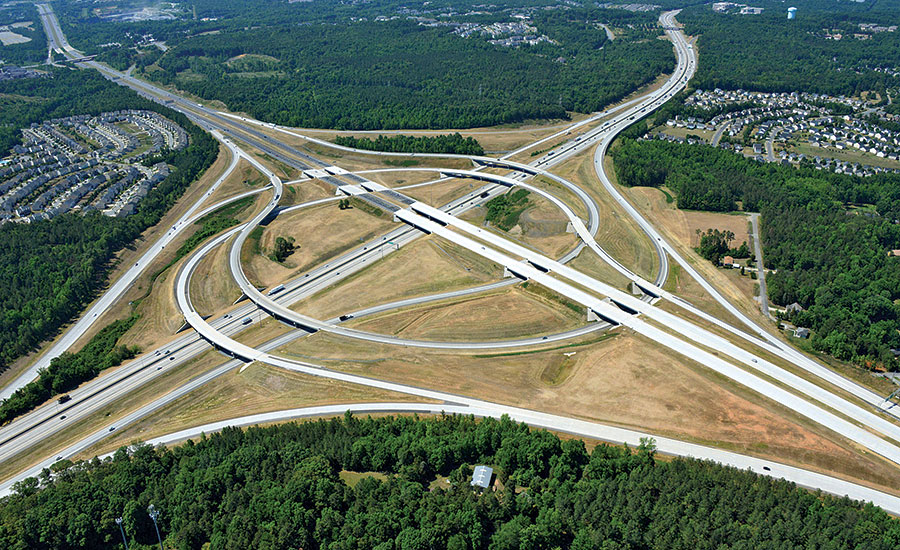
\includegraphics[width=0.4\textwidth]{images/loop-interchange.jpg}
\end{center}

Changes the nesting of loops to
coincide with the ordering of array elements in memory. 


\begin{center}
\vspace*{-1em}
\begin{minipage}{.39\textwidth}
  \begin{lstlisting}[language=Rust]
pub fn mul(mut a: [[i32; 8]; 4], c: i32) {
  for i in 0..7 {
     for j in 0..3 {
       a[i][j] = a[i][j] * c;
     }
  }
}
  \end{lstlisting}
  \end{minipage} $\hspace*{2em} \Longrightarrow \hspace*{2em}$ \begin{minipage}{.4\textwidth}
  \begin{lstlisting}[language=Rust]
pub fn mul(mut a: [[i32; 8]; 4], c: i32) {
  for j in 0..3 {
    for i in 0..7 {
      a[j][i] = a[j][i] * c;
    }
  }
}
  \end{lstlisting}
  \end{minipage}
  \end{center}
  A stackoverflow answer suggests that Rust is row-major
  (a[1][1] is beside a[1][2]) but that this is not
  guaranteed.
  
\end{frame}

\begin{frame}[fragile]
\frametitle{Loop Fusion}

This optimization is like the OpenMP collapse
construct; we transform
\begin{center}
\vspace*{-1em}
\begin{minipage}{.3\textwidth}
  \begin{lstlisting}[language=Rust]
    for i in 0..100 {
       a[i] = 4;
    }

    for i in 0..100 {
       b[i] = 7;
    }
  \end{lstlisting}
  \end{minipage} $\Longrightarrow \hspace*{2em}$ \begin{minipage}{.4\textwidth}
  \begin{lstlisting}[language=Rust]
    for i in 0..100 {
       a[i] = 4;
       b[i] = 7;
    }
  \end{lstlisting}
  \end{minipage}
  \end{center}
There's a trade-off between data locality and loop overhead.

Sometimes the inverse transformation, \emph{loop fission}, will
improve performance.

\end{frame}

\begin{frame}[fragile]
\frametitle{Loop-Invariant Code Motion}

 Also known as \emph{Loop hoisting},
this optimization moves calculations out of a loop. 
\begin{center}
\vspace*{-1em}
\begin{minipage}{.3\textwidth}
  \begin{lstlisting}[language=Rust]
for i in 0..100 {
    s = x * y;
    a[i] = s * i;
}
  \end{lstlisting}
  \end{minipage} $\Longrightarrow \hspace*{2em}$ \begin{minipage}{.4\textwidth}
  \begin{lstlisting}[language=Rust]
s = x * y;
for i in 0..100 {
    a[i] = s * i;
}
  \end{lstlisting}
  \end{minipage}
  \end{center}


This reduces the amount of work we have to do for each iteration of the loop.

\end{frame}


\begin{frame}[fragile]
\frametitle{Miscellaneous Low-Level Optimizations}

I used to talk about likely/unlikely branch prediction hints,
but Rust seems not keen to expose this. 

Rust does expose the \verb+#[cold]+
attribute, which you can use to mark a method as unlikely to be called (e.g. \texttt{panic}).


\end{frame}


\begin{frame}
\frametitle{Architecture-Specific}

LLVM can also generate code tuned to particular
processors. 

 You can specify this using {\tt  -C target-cpu} and {\tt -C target-feature}.

This will enable specific instructions that not all CPUs support (e.g. SSE4.2).

{\tt native} is a good target CPU if you run and compile on the same machine.

\noindent
Good to use on your local machine or your cloud servers, not ideal for code you ship to others.


\end{frame}



\begin{frame}
\frametitle{Interprocedural Analysis and Link-Time Optimizations}

``Are economies of scale real?''

In this context, does a
whole-program optimization really improve your program?


We'll start by first talking about some information that is critical for
whole-program optimizations.

\end{frame}


\begin{frame}
\frametitle{Alias and Pointer Analysis}

\begin{center}
	
\includegraphics[width=0.7\textwidth]{images/redstring.jpg}
\end{center}

It's all connected!

\end{frame}


\begin{frame}
\frametitle{Alias and Pointer Analysis}

Compiler optimizations often need
to know about what parts of memory each statement reads to.  

This is
easy when talking about scalar variables which are stored on the
stack. 

This is much harder when talking about pointers or arrays
(which can alias). 

This is much harder in conventional languages when talking about pointers or arrays, which can alias. 

The whole borrowing thing primarily controls aliasing.

\end{frame}

\begin{frame}
\frametitle{Alias Analysis}

When we know that two pointers don't alias, then we know that their
effects are independent, so it's correct to move things around.

Controlled aliasing makes it easier to reason about than in other languages.

Shape analysis
builds on pointer analysis to determine that data structures are indeed
trees rather than lists.


\end{frame}


\begin{frame}
\frametitle{Call Graph Analysis}

\begin{center}
	
\includegraphics[width=0.5\textwidth]{images/CallMeMaybe.png}
\end{center}

Many interprocedural analyses require accurate call graphs. 

\end{frame}


\begin{frame}
\frametitle{Call Graph}


A \alert{call graph} is a directed graph showing relationships between
functions. 

It's easy to compute a call graph when you have C-style
function calls. 

It's much harder when you have virtual methods, as in
C++ or Java, or even C function pointers. 

In particular, you need pointer
analysis information to construct the call graph.


\end{frame}


\begin{frame}
\frametitle{Devirtualization}

This optimization attempts to convert virtual function calls to direct calls.  

Virtual method calls have the potential to be slow, because there is effectively a branch to predict. 

(In general for Rust and \CPP, the program must read the object's vtable.) 

Plus, virtual calls impede other optimizations.

\end{frame}

\begin{frame}[fragile]
\frametitle{Devirtualization}

Compilers can help by doing sophisticated analyses to compute the call graph and by replacing virtual method calls with nonvirtual method calls.  


 \begin{lstlisting}[language=Rust]
     fn flag() -> bool { true }

     fn main() {
         let mut to: &dyn Foo = &Bar;
         if flag() { to = &Baz; }
         to.foo();
     }

     trait Foo { fn foo(&self) -> i32; }

     struct Bar;
     impl Foo for Bar {
         fn foo(&self) -> i32 { println!("bar"); 0 }
     }

     struct Baz;
     impl Foo for Baz {
         fn foo(&self) -> i32 { println!("baz"); 1 }
     }
  \end{lstlisting}

Devirtualization could eliminate vtable access; instead, we could just call {\tt Baz.foo()} 
directly. 

\end{frame}

\begin{frame}
\frametitle{Devirtualization}

`Rapid Type Analysis'' analyzes the entire program, observes that
only {\tt B} objects are ever instantiated, and enables devirtualization
of the {\tt b.m()} call.

\end{frame}

%%%%%%%%%%%%%%%%%%%%%%%%%%%%%%%%%%%%%%%%%%%%%%%%%%%%%%%%%%%%%%%%%%%%%%%%%%%%%%%%
\begin{frame}
  \frametitle{Inlining}

  

  We have seen the notion of inlining:
  \begin{itemize}
    \item Instructs the compiler to just insert the function code in-place,
      instead of calling the function.
    \item Hence, no function call overhead!
    \item Compilers can also do better---context-sensitive---operations they couldn't
      have done before.
  \end{itemize}
  \vfill
\end{frame}

\begin{frame}
\frametitle{Inline Commands}

In Rust, you can tell the compiler to inline a function using an annotation:
\begin{itemize}
 \item \#[inline] hints the compiler to perform an inline expansion.
 \item \#[inline(always)] asks the compiler to always perform an inline expansion.
 \item \#[inline(never)] asks the compiler to never perform an inline expansion.
\end{itemize}

  
  No overhead\ldots~ sounds like better performance\ldots~ \\let's inline everything!
  
\end{frame}
%%%%%%%%%%%%%%%%%%%%%%%%%%%%%%%%%%%%%%%%%%%%%%%%%%%%%%%%%%%%%%%%%%%%%%%%%%%%%%%%

%%%%%%%%%%%%%%%%%%%%%%%%%%%%%%%%%%%%%%%%%%%%%%%%%%%%%%%%%%%%%%%%%%%%%%%%%%%%%%%%
\begin{frame}
  \frametitle{The Other Side of Inlining}

  

  One big downside:
  \begin{itemize}
    \item Your program size is going to increase.
  \end{itemize}
   This is worse than you think:
      \begin{itemize}
        \item Fewer cache hits.
        \item More trips to memory.
      \end{itemize}
   Some inlines can grow very rapidly (C++ extended constructors).\\[1em]
  Just from this your performance may go down easily.
  
\end{frame}
%%%%%%%%%%%%%%%%%%%%%%%%%%%%%%%%%%%%%%%%%%%%%%%%%%%%%%%%%%%%%%%%%%%%%%%%%%%%%%%%

%%%%%%%%%%%%%%%%%%%%%%%%%%%%%%%%%%%%%%%%%%%%%%%%%%%%%%%%%%%%%%%%%%%%%%%%%%%%%%%%
\begin{frame}
  \frametitle{Compilers on Inlining}

  

  Inlining is merely a suggestion to compilers.\\
  They may ignore you.\\[1em]

  For example:
n  \begin{itemize}
    \item taking the address of an ``inline'' function and using it; or
    \item virtual functions (in C++),
  \end{itemize}
  will get you ignored quite fast.
  
\end{frame}
%%%%%%%%%%%%%%%%%%%%%%%%%%%%%%%%%%%%%%%%%%%%%%%%%%%%%%%%%%%%%%%%%%%%%%%%%%%%%%%%

%%%%%%%%%%%%%%%%%%%%%%%%%%%%%%%%%%%%%%%%%%%%%%%%%%%%%%%%%%%%%%%%%%%%%%%%%%%%%%%%
\begin{frame}
  \frametitle{From a Usability Point-of-View}

  
  Debugging is more difficult (e.g. you can't set a breakpoint in a function that
  doesn't actually exist).
  \begin{itemize}
    \item Most compilers simply won't inline code with debugging symbols on.
    \item Some do, but typically it's more of a pain.
  \end{itemize}~\\[1em]

  Library design:
  \begin{itemize}
    \item If you change any inline function in your library, any users
      of that library have to {\bf recompile} their program if the
      library updates. (non-binary-compatible change!)
  \end{itemize}
  Not a problem for non-inlined functions---programs execute the new function
      dynamically at runtime.

  
\end{frame}
%%%%%%%%%%%%%%%%%%%%%%%%%%%%%%%%%%%%%%%%%%%%%%%%%%%%%%%%%%%%%%%%%%%%%%%%%%%%%%%%


\begin{frame}
\frametitle{Inlining}

 Compilers can inline following compiler directives, but usually more based on heuristics. 
 
 Devirtualization enables more inlining. 
 

\end{frame}

\begin{frame}[fragile]
\frametitle{Devirtualization and Inlining}

Obviously, inlining and devirtualization require call graphs. 

But so
does any analysis that needs to know about the heap effects of
functions that get called.


{\small
\begin{lstlisting}[language=Rust]
    static mut N:i32 = 5;

    fn f() { }

    fn main() {
      unsafe { 
        N = 2;
        f();
        println!("{}", N);  
      }
    }
    \end{lstlisting}
}

We could propagate the constant value 2 to the print statement,
as long as we know that {\tt f()} does not write to {\tt N}.

But idiomatic Rust helps us here.

\end{frame}

\begin{frame}[fragile]
\frametitle{Tail Recursion Elimination}

This optimization is mandatory in some functional languages; we replace a call by a {\tt goto} at the compiler level.

{\small
\begin{lstlisting}[language=Rust]
pub fn fibonacci(n: u64) -> u64 {
    fn fibonacci_lr(n: u64, a: u64, b: u64) -> u64 {
        match n {
            0 => a,
            _ => fibonacci_lr(n - 1, a + b, a),
        }
    }
    fibonacci_lr(n, 1, 0)
}
\end{lstlisting}
}
Here, \texttt{fibonacci\_lr} doesn't need to return control to its caller
(because the recursive call is in tail position. 

This avoids function call overhead and reduces call stack use.
\end{frame}


\begin{frame}
\frametitle{Link-Time Optimization}

\begin{center}
	
\includegraphics[width=\textwidth]{images/sadzelda.jpg}
\end{center}

``I've spent a hundred years trying to hold back Calamity Ganon and you've spent your time doing WHAT?''

\end{frame}


\begin{frame}
\frametitle{Link-Time Optimization}


Biggest challenge for interprocedural optimizations = scalability, so 
it fits right in as a topic of discussion for this course.

An outline of interprocedural optimization:

\begin{itemize}
\item local generation (parallelizable)
\item whole-program analysis (hard to parallelize!)
\item local transformations (parallelizable)
\end{itemize}

\end{frame}


\begin{frame}
\frametitle{Transformations in Code}

Transformations:

\begin{itemize}
\item global decisions, local transformations:
\begin{itemize}
\item devirtualization
\item dead variable elimination/dead function elimination
\item field reordering, struct splitting/reorganization
\end{itemize}
\item global decisions, global transformations:
\begin{itemize}
\item cross-module inlining
\item virtual function inlining
\item interprocedural constant propagation
\end{itemize}
\end{itemize}


\end{frame}


\begin{frame}[fragile]
\frametitle{Whole Program Analysis}

The interesting issues arise from making the whole-program analysis scalable. 

\begin{verbatim}
-----------------------------------------------------------
Language                files        comment           code
-----------------------------------------------------------

[Chromium] C++          44991        1405276       11102212
[Firefox] C++           10973         605158        4467943
[Linux] C               26238        2573558       13092340
\end{verbatim}


Whole-program analysis requires that all of 
this code (in IR) be available to the analysis \& some summary of the code be in memory,  along with the call graph.

\end{frame}


\begin{frame}
\frametitle{Whole Program Analysis}

\large


Whole-program analysis $\Rightarrow$ any part of the program may affect other parts. 

First problem: getting it into memory; loading the IR for tens of millions of lines of code is a non-starter.


Clearly, anything that is more expensive than linear time can cause problems. 

Partitioning the program can help.


\end{frame}


\begin{frame}
\frametitle{gcc Whole Program Analysis}

{\Large How did gcc get better?  Avoiding unnecessary work. }

\begin{itemize}
\item gcc 4.5: initial version of LTO;
\item gcc 4.6: parallelization; partitioning of the call graph (put closely-related functions together, approximate functions in other partitions); the bottleneck: streaming in types and declarations;
\item gcc 4.7--4.9: improve build times, memory usage [``chasing unnecessary data away''.]
\end{itemize}

Today's gcc, with {\tt -flto}, does work and includes
optimizations including constant propagation and function
specialization.

LLVM LTO can, however, optimize across source languages.

\end{frame}



\begin{frame}
\frametitle{It Works!}

\Large


gcc LTO gives $\sim$ 3--5\% perf improvements (good per compiler experts).


Developers can shift attention from 
manual factoring to letting compiler do it.

\end{frame}



\end{document}

